\label{popmodel}
\subsection{Introduction}
Object-oriented programming provides high level abstractions for software
engineering. In addition, the nature of objects makes them ideal
structures to distribute data and executable codes over heterogeneous
distributed hardware and to make them interact between each other.
Nevertheless, two questions remain:

\begin{itemize}

\item Question 1: which objects should run remotely?

\item Question 2: where does each remote object live?

\end{itemize}

The answers, of course, depend on what these objects do and how
they interact with each other and with the outside world. In other
words, we need to know the communication and the computation
requirements of objects. The parallel object model presented in this
chapter provides an object-oriented approach for requirement-driven high
performance applications in a distributed heterogeneous environment.


\subsection{Parallel Object Model}
POP stands for {\it Parallel Object Programming}, and POP parallel objects are
generalizations of traditional sequential objects. POP-Java is an
extension of Java that implements the POP model. POP-Java instantiates
parallel objects transparently and dynamically, assigning suitable
resources to objects. POP-Java also offers various mechanisms to specify
different ways to do method invocations. Parallel objects have all the properties
of traditional objects plus the following ones:

\begin{itemize}

\item Parallel objects are shareable. References to parallel objects can
       be passed to any other parallel object. This property is described in section \ref{shareable}.

\item Syntactically, invocations on parallel objects are identical to
       invocations on traditional sequential objects. However, parallel
       objects support various method invocation semantics: synchronous
       or asynchronous, and sequential, mutex or concurrent. These
       semantics are explained in section \ref{semantic}.

\item Parallel objects can be located on remote resources in separate
       address spaces. Parallel objects allocations are transparent to
       the programmer. The object allocation is presented in section
       \ref{allocation}.

\item Each parallel object has the ability to dynamically describe its
       resource requirement during its lifetime. This feature is
       discussed in detail in section \ref{requirement}

\end{itemize}

As for traditional objects, parallel objects are active only when they execute
a method (non active object semantic). Therefore, communication between
parallel objects are realized thank to remote methods invocation.


\pagebreak
\subsection{Shareable Parallel Objects}
\label{shareable}
Parallel objects are shareable. This means that the reference of a
parallel object can be shared by several other parallel objects.
Sharing references of parallel objects are useful in many cases.
For example, figure[\ref{fig_use_scenario}] illustrates a scenario of
using shared parallel objects: \texttt{input} and \texttt{output}
parallel objects are shareable among \texttt{worker} objects.
A \texttt{worker} gets work
units from \texttt{input} which is located on the data server, performs
the computation and stores the results in the \texttt{output} located at
the user workstation. The results from different \texttt{worker} objects
can be automatically synthesized and visualized inside \texttt{output}.


\begin{figure}[ht]
	\caption{A scenario using shared parallel objects}
  	\centering
	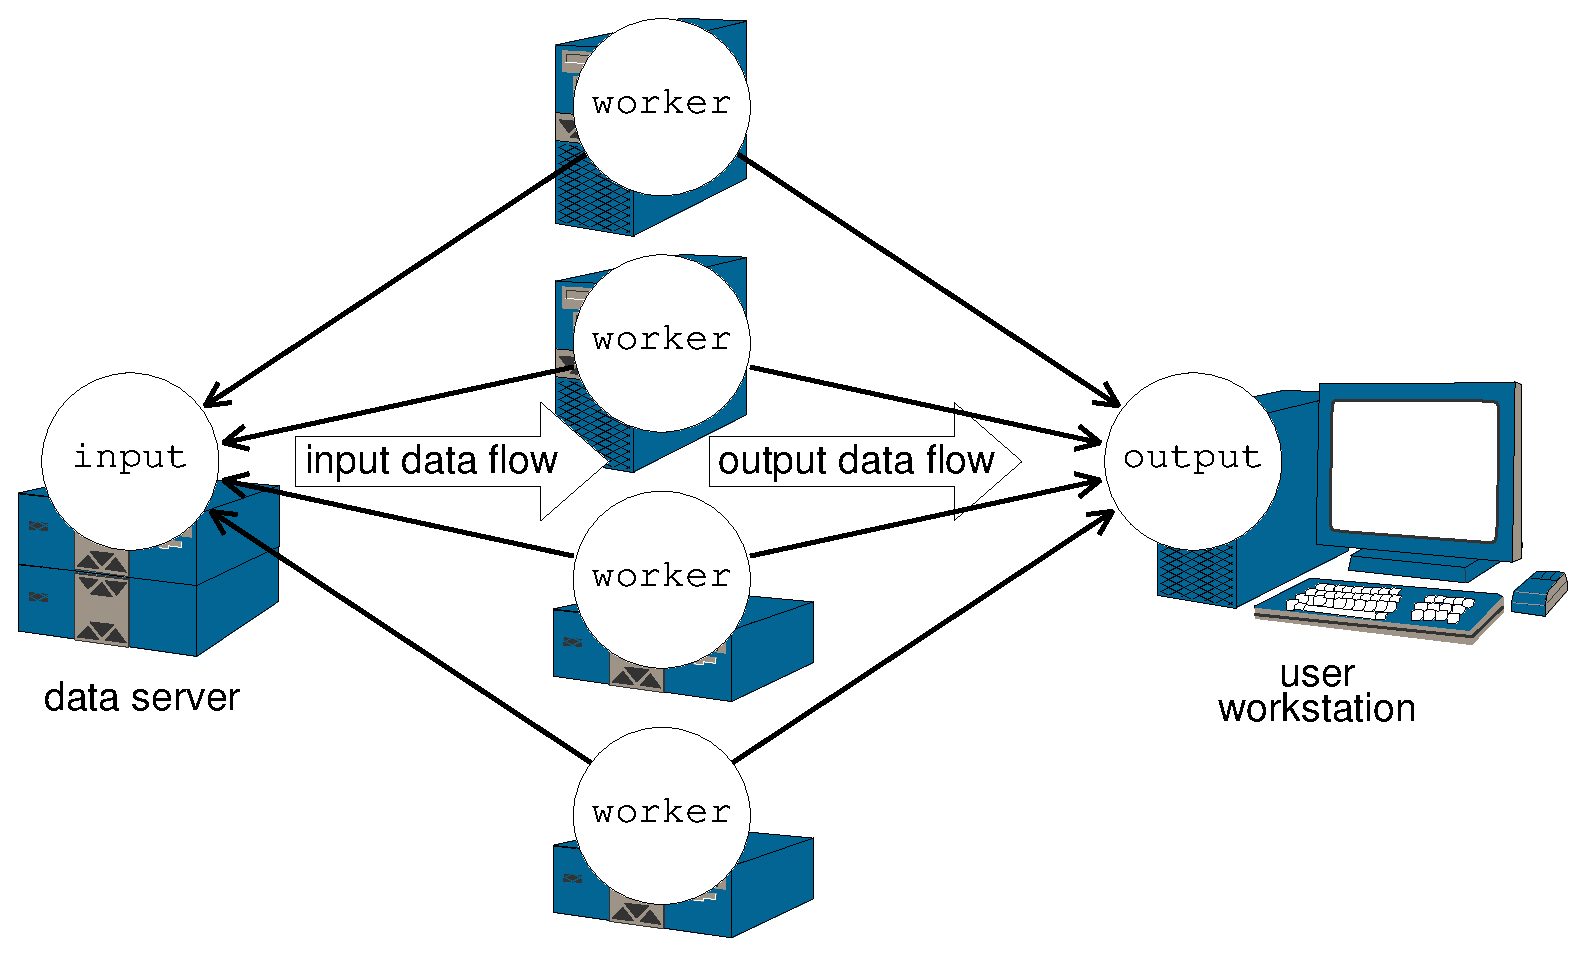
\includegraphics[scale=0.5]{fig_use_scenario.eps}
	\label{fig_use_scenario}
\end{figure}


To share the reference of a parallel object, POP-Java allows parallel objects
to be arbitrarily passed from one place to another as arguments of method
invocations.

\pagebreak
\subsection{Invocations semantics}
\label{semantic}
Syntactically, method invocations on parallel objects are identical to those
on traditional sequential objects. However, to each method of a parallel
object, one can associate different invocation semantics. Invocation
semantics are specified by programmers when declaring methods of
parallel objects. These semantics define different behaviors for the
execution of the method as described below (example of syntax in chapter \ref{dev})

\begin{itemize}

\item \emphasis{Interface semantics}, the semantics that affect the caller
of the method:
	\subitem \textbf{Synchronous invocation}: the caller waits until the
	execution of the called method on the remote object is terminated.
  This corresponds to the traditional method invocation.

	\subitem \textbf{Asynchronous invocation}: the invocation returns
	immediately after sending the request to the remote object.
	Asynchronous invocation is important to exploit the parallelism.
	However, as the caller does not wait the end of the execution of the
	called method, no computing result is available. This excludes
	asynchronous invocations from producing results. Results can be
	actively returned to the caller object using a callback to the caller.
	To do so the called object must have a reference to the caller object.
	This reference can be passed as an argument to the called method
	(see figure[\ref{fig_inv_async}]).




\begin{figure}[ht]
	\caption{Callback method returning values from an asynchronous call}
  	\centering
	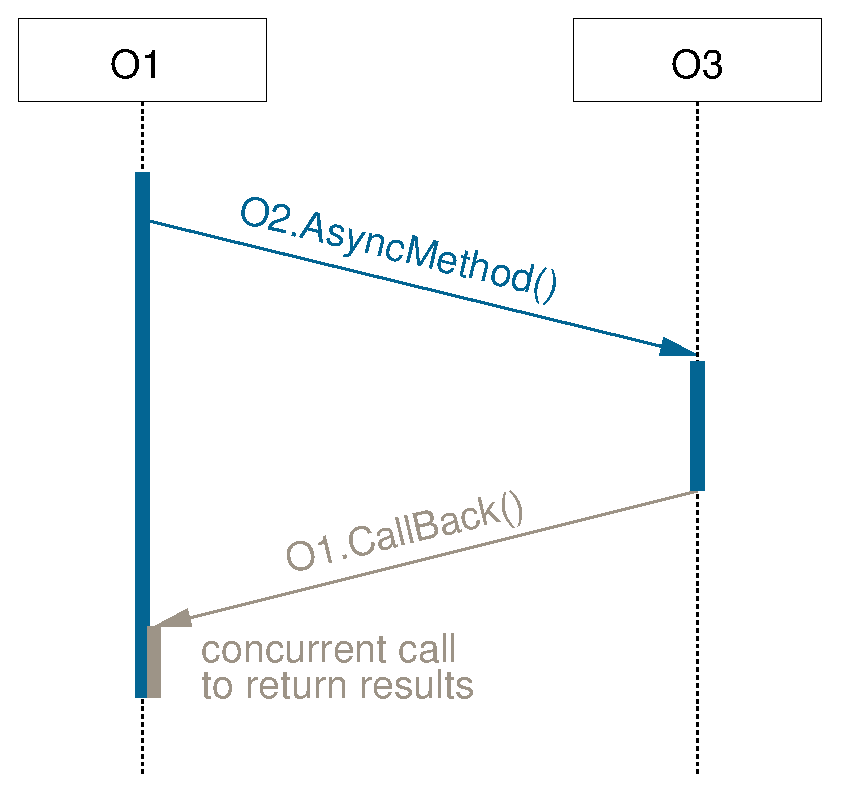
\includegraphics[scale=0.5]{fig_inv_async.eps}
	\label{fig_inv_async}
\end{figure}



\item \emphasis{Object-side semantics}, the semantics that affect the order
 of the execution of methods in the called parallel object:

	\subitem \textbf{A mutex call} is executed after completion of all calls previously arrived.
	
	\subitem \textbf{A sequential call} is executed after completion of all sequential and
	mutex calls previously arrived.

	\subitem \textbf{A concurrent call} can be executed concurrently (time sharing) with other
	concurrent or sequential calls, except if mutex calls are pending or executing.
	In the later case he is executed after completion of all mutex calls previously
	arrived.

\end{itemize}

In a nutshell, different object-side invocation semantics can be
expressed in terms of atomicity and execution order. The mutex
invocation semantics guarantees the global order and the atomicity of
all method calls. The sequential invocation semantics guarantees only
the execution order of sequential methods. Concurrent invocation
semantics guarantees neither the order nor the atomicity.


\begin{figure}[ht]
	\caption{Example of different invocation requests}
  	\centering
	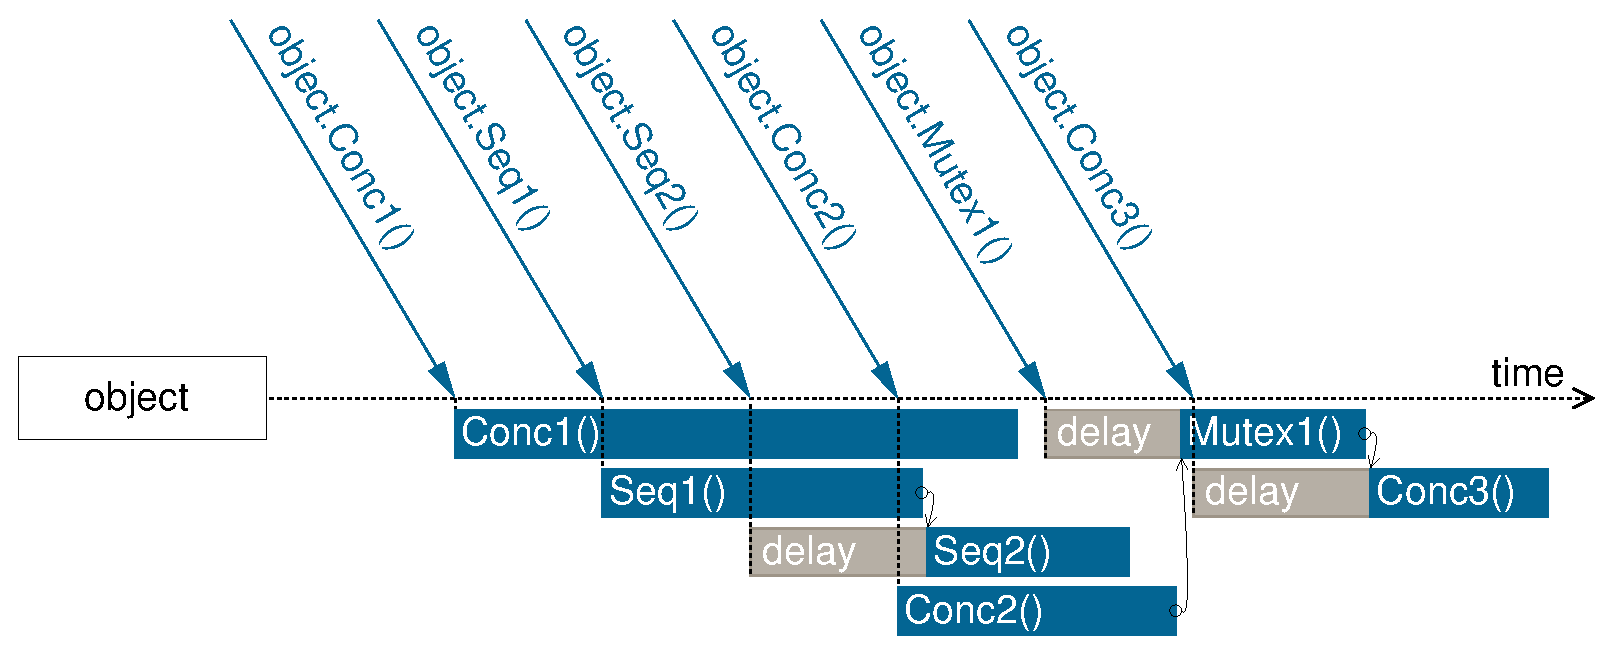
\includegraphics[scale=0.5]{fig_inv_semantics.eps}
	\label{fig_inv_semantics}
\end{figure}


Figure[\ref{fig_inv_semantics}] illustrates different method invocation
semantics. Sequential invocation \texttt{Seq1()} is served immediately,
running concurrently with \texttt{Conc1()}. Although the sequential
invocation \texttt{Seq2()} arrives before the concurrent invocation
\texttt{Conc2()}, it is delayed due to the current execution of
\texttt{Seq1()} (no order between concurrent and sequential invocations).
When the mutex invocation \texttt{Mutex1()} arrives, it has to wait for
other running methods to finish. During this waiting, it also blocks
other invocation requests arriving afterward (\texttt{Conc3()}) until
the mutex invocation request completes its execution (atomicity and
barrier).


\subsection{Parallel Object Allocation}
\label{allocation}
The first step to allocate a new object is the selection of an adequate
placeholder. The second step is the object creation itself. Similarly,
when an object is no longer in use, it must be destroyed in order to
release the resources it is occupying in its placeholder. The POP-C++
runtime system provides automatic placeholder selection, object
allocation, and object destruction. This automatic features result in a
dynamic usage of computational resources and gives to the applications
the ability to adapt to the changes in both the environment and the user
behavior.\s

The creation of POP-Java parallel objects is driven by high-level
requirements on the resources where the object should lie (see section
\ref{requirement}). If the programmer specifies these requirements
they are taken into consideration by the runtime system for the transparent 
object allocation. The allocation process consists of three phases: first, the system finds a suitable resource, where the
object will lie; then the object code is transmitted and executed on
that resource; and finally, the corresponding interface is created and
connected to the object.


\subsection{Requirement-driven parallel objects}
\label{requirement}
Parallel processing is increasingly being done using distributed
systems, with a strong tendency towards web and global computing.
Efficiently extract high performance from highly heterogeneous and
dynamic distributed environments is a challenge today. POP-C++ and POP-Java were
conceived under the belief that for such environments, high performance
can only be obtained if the two following conditions are satisfied:

\begin{itemize}

\item The application should be able to adapt to the environment;

\item The programming environment should somehow enables objects
to describe their resource requirements.

\end{itemize}

The application adaptation to the environment can be fulfilled by
multilevel parallelism, dynamic utilization of resources or adaptive
task size partitioning. One solution is to dynamically create parallel
objects on demand.

Resource requirements can be expressed by the quality of service that
objects require from the environment. Most of the systems offering
quality of service focus on low-level aspects, such as network bandwidth
reservation or real-time scheduling. Both POP-C++ and POP-Java integrate the programmer
requirements into parallel objects in the form of high-level resource
descriptions. Each parallel object is associated with an object
description that depicts the characteristics of the resources needed to
execute the object. The resource requirements in object descriptions are
expressed in terms of:

\begin{itemize}

\item Resource (host) name (low level description, mainly used to
develop system services).

\item The maximum computing power that the object needs (expressed in
MFlops).

\item The maximum amount of memory that the parallel object consumes.

\item The expected communication bandwidth and latency.

\item The preferred communication protocol.

\item The preferred encoding protocol.


\end{itemize}

An object description can contain several items. Each item corresponds
to a type of characteristics of the desired resource. The item is
classified into two types: strict item and non-strict item. A strict
item means that the designated requirement must be fully satisfied. If
no satisfying resource is available, the allocation of parallel object
fails. Non-strict items, on the other hand, give the system more freedom
in selecting a resource. Resource that partially match the requirements
are acceptable although a full qualification resource is  preferable.
For example, a certain object has a preferred performance 150MFlops
although 100MFlops is acceptable (non-strict item), but it need memory
storage of at least 128MB (strict item).\s

The construction of object descriptions occurs during the parallel
object creation. The programmer can provide an object description to
each object constructor. The object descriptions can be parametrized by
the arguments of the constructor. Object descriptions are used by the
runtime system to select an appropriate resource for the object. Some example 
of the syntax of object descriptions can be found in the section \ref{dev:objdesc}.\s

It can occur that, due to some changes on the object data or some
increase of the computation demand, an object description needs to be
re-adjusted during the life time of the parallel object. If the new
requirement exceeds some threshold, the adjustment could cause the
object migration. The current implementations of POP-C++ and POP-Java do not support
object migration yet.
